% This is samplepaper.tex, a sample chapter demonstrating the
% LLNCS macro package for Springer Computer Science proceedings;
% Version 2.21 of 2022/01/12
%
\documentclass[runningheads]{llncs}
%
\usepackage[T1]{fontenc}
% T1 fonts will be used to generate the final print and online PDFs,
% so please use T1 fonts in your manuscript whenever possible.
% Other font encondings may result in incorrect characters.
%
\usepackage{graphicx}
\usepackage{amsmath}
\usepackage{float}
\usepackage{marvosym}
\raggedbottom
\setlength{\floatsep}{4pt plus 2pt minus 2pt}
\setlength{\textfloatsep}{6pt plus 2pt minus 2pt}
\setlength{\intextsep}{4pt plus 2pt minus 2pt}
% Used for displaying a sample figure. If possible, figure files should
% be included in EPS format.
%
% If you use the hyperref package, please uncomment the following two lines
% to display URLs in blue roman font according to Springer's eBook style:
%\usepackage{color}
%\renewcommand\UrlFont{\color{blue}\rmfamily}
%\urlstyle{rm}
%
\begin{document}
%
\title{Model-free multi-agent reinforcement learning
simulation of the influence of empathy on the
sustainability of agents' consumption in a
common-pool resource dilemma}
%
\titlerunning{MARL simulation of empathy}
% If the paper title is too long for the running head, you can set
% an abbreviated paper title here
%
\author{Jérôme Iste\inst{1,2} \and
Evann Rabeau\inst{2}\textsuperscript{(\Letter)} \and
Mehdi Khamassi\inst{1} \and
Ismael T. Freire\inst{1}
}
%
\authorrunning{Iste et al.}
% First names are abbreviated in the running head.
% If there are more than two authors, 'et al.' is used.
%
\institute{Institute of Intelligent Systems and Robotics, CNRS, Sorbonne University, Paris, France \and
Université Paris Cité, Paris, France\\
\email{evann.rabeau@etu.u-paris.fr}}

%
\maketitle              % typeset the header of the contribution
%
\begin{abstract}
The escalating ecological crisis accentuates the need for effective strategies to mitigate resource depletion. This study introduces a novel reinforcement-learning model of empathy, integrating its cognitive and motivational components, and applies it in a multi-agent common-pool resource setting to investigate computational hypotheses about the role of empathy---defined as the capacity to integrate others' emotional states into one's decisions and a drive to promote their well-being---in common-pool resource dilemmas. We examine how empathy (empathetic agents vs. selfish agents) influences economic equity and environmental sustainability. Our findings suggest that empathy, as conceptualized here, may reduce overconsumption, but may not lead to a fairer distribution of resources. These results highlight empathy as a potentially key mechanism for fostering cooperative behavior and addressing environmental challenges.

\keywords{MARL \and Empathy \and Common-Pool Resource Dilemma}
\end{abstract}
%
%
%
\newpage
\section{Introduction}
\subsection{Empathy}
The Tragedy of the Commons, introduced by \cite{hardinTragedyCommonsPopulation1968}, describes how population growth and resource demand can lead to overexploitation of shared resources. Amid the current environmental crisis, understanding psycho-social properties and organisational frameworks to limit the risk of the Tragedy in humans is becoming existentially crucial. This research seeks to identify theoretical implications of the current understanding of empathy on resource consumption and its fairness with the use of a decentralized model-free multi-agent reinforcement learning framework.
Economists study this issue through the paradigm of common-pool resource dilemmas, where groups decide how much of a shared resource to extract, but individuals can exploit more or less of the resource than the agreed-upon amount \cite{patelModellingCooperationCompetition2021}. Common-pool resources are defined by two properties \cite{ostromRevisitingCommonsLocal1999,perolatMultiagentReinforcementLearning2017}:
(1) Non-exclusivity: agents cannot easily be excluded from consuming the resources.
(2) Subtractability: agent's consumption reduces the availability to others.
Classic economic theory predicts that rational agents, aiming to maximise their marginal utility, converge towards a Nash Equilibrium \cite{nashEquilibriumPointsPerson1950}. Cumulative exploitation leads to resource depletion and suboptimal outcomes for individuals and the group \cite{patelModellingCooperationCompetition2021}. This reflects crucial tensions between self-interest and collective welfare, and between short-term and long-term interests \cite{vanlangeHowWeCan2008}.


\subsection{Multi-agent reinforcement learning}
Multi-agent reinforcement learning (MARL) has increasingly been used as a computational framework for modelling socio-cognitive phenomena in interactive environments \cite{gronauerMultiagentDeepReinforcement2022} and has even been applied to model multi-agent behaviors in a tragedy of the commons scenario \cite{perolatMultiagentReinforcementLearning2017}.
 To study common-pool resources and other social dilemmas, decentralized learning Model-Free (MF) agents are frequently used, thus framing these dilemmas as reward maximization problems \cite{perolatMultiagentReinforcementLearning2017,wangEvolvingIntrinsicMotivations2018,zhuDeepMultiagentReinforcement2019}.
 MF agents incrementally update their policies based on direct reward experiences, linking them to procedural learning \cite{kosterModelfreeConventionsMultiagent2020,massiModelbasedModelfreeReplay2022}. In contrast, model-based agents integrate an internal representation of the environment, allowing them to simulate outcomes and adapt strategies more flexibly to changes. Although this approach allows simulation of decision-making and planning capabilities, it demands greater computational resources and assumes advanced agent capabilities \cite{massiModelbasedModelfreeReplay2022}.

MF-MARL simulations have recently been used to understand the dilemmas of common-pool resources. \cite{perolatMultiagentReinforcementLearning2017} demonstrated that allowing agents to stop others for a set duration, thus temporarily limiting the number of active foraging ones, allowed the system to reach an equilibrium. They observed three phases of the system: naïvety (i.e., increased utility but decreased sustainability), tragedy (i.e., declines in sustainability, peace, and utility), and maturity (i.e., utility and sustainability improved steadily despite reduced freezing action selection and stable equality). Similarly, \cite{zhuDeepMultiagentReinforcement2019} experimentally demonstrated that larger groups depleted resources faster, but that higher valuation of sustainability parameter in the reward function could mitigate that effect. Finally, \cite{kosterModelfreeConventionsMultiagent2020} observed that agents with heterogeneous preferences formed bottom-up conventions. They prioritized maximizing others' optimality over their hypothetical gain. This showcases emergent cooperative behaviors. To our knowledge, no existing work has yet proposed a way to model empathetic processes within a MARL framework. We now turn to examining key properties that may influence the likelihood of a Tragedy of the Commons, with a particular focus on mechanisms like empathy, through the observation of others' states and the valuation of their utility.

\subsection{Determinants of the Tragedy}
\subsubsection{Top-down organizational determinants.}
From a governance system and economic perspective, effective governance requires balancing resource access with sustainable consumption incentives, addressing both collective needs and individual use \cite{ostromRevisitingCommonsLocal1999,ostromGeneralFrameworkAnalyzing2009}. Ostrom \cite{ostromGeneralFrameworkAnalyzing2009} identified five interacting conditions of effective management of common-pool resources at the local and regional levels. First, users should benefit from organizing collectively. Second, reliable and valid indicators of resource conditions should enable users to assess long-term costs and benefits. Third, users must anticipate that the collective benefits outweigh the personal costs. Fourth, there should be sufficient trust among users or low-cost mechanisms to monitor and sanction non-compliance. Finally, users should actively participate in the decision-making process. In addition, \cite{ostromGeneralFrameworkAnalyzing2009} introduced a comprehensive framework to analyze the sustainability of socioecological systems. This framework links users, governance systems, resource systems, and resource units with their outcomes and interactions while considering the ecological, social, and economic contexts.

\subsubsection{Group and interaction level determinants}
Although institutional frameworks are essential for managing individual resource consumption, social interactions at the local level also play a critical role in promoting sustainable resource use. In their survey of Maasai pastoralists, \cite{rabinovichProtectingCommonsPredictors2020} observed that group membership was associated with the prioritization of collective outcomes and resource protection. Similarly, \cite{cuadradoRoleProsocialnessTrust2017} observed that in a multiplayer farming game, those who could communicate and had a secondary common goal of maximizing global profit chose less selfish irrigation strategies and obtained greater individual gains. Furthermore, \cite{decaroSynergisticEffectsVoting2015,decaroMotivationalFoundationsCommunication2021} observed that in a blind common-pool resources study, democratic decisions and social rewards favored the respect for negotiated rules and performance. They increased needs-satisfaction, intrinsic motivation, and trust with effects lasting even after communication was interrupted. The humanistic rational choice theory explains these results by proposing that a virtuous cycle of conditional cooperative self-governance can emerge from the satisfaction of three core psychosocial processes: (1) fundamental need satisfaction, (2) institutional internalisation and acceptance, and (3) group cohesion \cite{decaroMotivationalFoundationsCommunication2021}. Along this view, fundamental needs are evolved socio-psychological elements essential to human well-being: procedural justice (fairness), self-determination, security, efficacy and understanding, social acceptance and meaningful social relationships, and fair distribution of costs/benefits of governance.

\subsubsection{Individual-level determinants}
In the context of behavioral interventions, researchers have identified various psychosocial variables—such as values, beliefs, and social norms—as key predictors of pro-environmental behavior \cite{fornaraExtendedValueBeliefNormTheory2020,guoResidentialElectricityConsumption2018,liWhatInfluencesIndividuals2019,sussmanProEnvironmentalValuesMatter2016}. To integrate these determinants, Thiermann and Sheate \cite{thiermannMotivatingIndividualsSocial2020} proposed the two-pathway model of pro-environmental behavior that connects the Value-Belief-Norm (VBN) model \cite{sternValuebeliefnormTheorySupport1999}, the Theory of Planned Behavior (TPB; \cite{ajzenTheoryPlannedBehavior1991}), habits, and empathetic processes. The normative pathway links values and intentions to behavior. In contrast, the relational pathway highlights the influence of empathy, compassion, and connectedness with nature.
In a related perspective, \cite{moreno-casasEthicsCareTragedy2021} suggest that the ethics of care, grounded in empathic recognition of others' needs, can mitigate the tragedy of the commons by fostering cooperative behavior and concern for collective well-being. Similarly, the dual interest theory developed by \cite{lynneTheoreticalFoundationEmpathy2016} posits that individuals may derive utility through empathic processes, allowing empathy to curb self-interest and promote sustainable behavior.
From an evolutionary standpoint, empathy may have been selected as an adaptive trait that enhanced group-based foraging strategies and cooperation, thereby supporting human survival and reproduction (\cite{tomaselloTwoKeySteps2012}). Over time, environmental pressures favored empathy and affective signaling as mechanisms for promoting group cohesion, moral concern, and the sharing of resources \cite{cuffEmpathyReviewConcept2016,decetyEmergenceEmpathyDevelopmental2021,tomaselloOriginsHumanCooperation2013}. Having established empathy as a potentially key determinant of pro-environmental behaviors, the next section presents a theoretical framework to define it.



\subsection{Defining empathy}
The literature review above emphasized how empathy can be considered as an adaptive trait that may have enhanced group-based cooperation. Nevertheless, in the psychology literature, multiple definitions of empathy exist, and it is important to be clear about what we mean by empathy here before being able to formalize a tentative mechanism for its influence on reinforcement learning processes.

\subsubsection{The object of empathy: what are emotions?}
Emotions, the primary objects of empathetic processes, can be defined as categorical entities (e.g., fear, joy) composed of five components: phenomenological experience, physiological response, expressive behaviors, behavioral tendencies, and emotivational goals \cite{rosemanEmotionalBehaviorsEmotivational2011}. Alternatively, emotions can be described dimensionally, along axes such as valence and activation within a circumplex model \cite{russellCoreAffectPsychological2003,rosemanEmotionalBehaviorsEmotivational2011}. Appraisal theories propose that emotions result from rapid evaluations of stimuli based on criteria such as goal relevance and perceived control \cite{broschCommentAppraisingBrain2013,moorsPowerGoalDirectedProcesses2017}. Thus, depending on agents' goals, both positive and negative emotions may be induced by resource consumption and depletion. Emotional expressions, especially those associated with valence (e.g., distress or satisfaction), can act as social signals and influence others' decisions regarding resource sharing, particularly in common-pool dilemmas \cite{lynneTheoreticalFoundationEmpathy2016}.

\subsubsection{Processing others' emotions: what is empathy?}
Empathy is a complex construct that lacks a universally accepted definition and is often conflated with related concepts such as sympathy, emotional contagion, compassion, and prosociality \cite{cuffEmpathyReviewConcept2016}. Nonetheless, it is generally agreed to involve both understanding and sharing the emotional state of another person, with the recognition that the other is the source. Empathy arises from the interaction between trait capacities and situational influences, combining automatic emotion-eliciting processes and top-down control \cite{cuffEmpathyReviewConcept2016}. This results in an emotional experience aligned with the perception of another person's emotion, while maintaining self-other distinction.

\subsubsection{Three components of empathy: cognitive, affective, and motivational}
Empathy is commonly described as comprising three components, each supported by distinct neural systems:
\begin{itemize}
	\item \textbf{Cognitive empathy}: The capacity to understand or imagine what another person is feeling.
	\item \textbf{Affective empathy}: The capacity to share or resonate with the emotional state of another person \cite{bosnjakovicEmpathyConceptsTheories2018,dewaalMammalianEmpathyBehavioural2017}. Affective empathy is distinguished from emotional contagion by the awareness that the emotion originates in another person, not the self. The role of mirror neurons in empathy remains debated, with mixed empirical results \cite{bekkaliPutativeMirrorNeuron2021,boniniMirrorNeurons302022}. Both cognitive and affective empathy induce similar emotion-specific neural activations, with differences related to self-other differentiation \cite{bernhardtNeuralBasisEmpathy2012,dvashTheoryMindEmpathy2014}.
	\item \textbf{Motivational empathy (empathic concern)}: The drive to care for others' well-being, often considered a third and independent component, or as a form of prosocial motivation encompassing sympathy and compassion \cite{dewaalMammalianEmpathyBehavioural2017,decetyEmergenceEmpathyDevelopmental2021}.
\end{itemize}

While cognitive and affective empathy allow us to have a correct estimate of the other's utility, they do not intrinsically influence our behavior. Following utility based calculus theory of action selection and the empathic-altruistic hypothesis \cite{Batson01041991,batson2022empathy}, the empathic concern or motivational component is the key to drive behavior from the proper estimation of the others' states.

\subsection{Theoretical Hypotheses}
Drawing from social psychology models, economic theories \cite{lynneTheoreticalFoundationEmpathy2016,thiermannMotivatingIndividualsSocial2020}, and findings from MARL research on prosocial behavior \cite{yuEmotionalMultiagentReinforcement2015}, four theoretical hypotheses (TH) are proposed, organized around two objectives.

Objective 1: To study the independent and combined contributions of the components of empathy. We expect that both cognitive empathy and motivational empathy will independently reduce resource overconsumption, thereby delaying depletion and extending episode length, with their combination producing the strongest effect on sustainability (TH1). Additionally, we expect that both components will independently promote fairer resource access, with their interaction yielding the most equitable distribution outcomes (TH2).

Objective 2: To examine the parametric modulation of the motivational empathy component across a continuous range of altruistic valuation. We expect a positive monotonic relationship between the degree of altruistic motivation and sustainability, such that higher levels of motivational empathy will be associated with longer episodes before resource depletion (TH3). Similarly, we expect that increasing altruistic motivation will produce progressively more equitable patterns of resource consumption across agents (TH4).



\section{Method}
\subsection{Simulation Framework}
\subsubsection{Environment}

We model the problem as a partially observable stochastic game defined as a tuple
$\langle N, S, A, T, R, \Omega, O \rangle$.
$N = 6$ agents interact over a shared depletable common-pool resource.
The state space $S$ is defined by the current resource level $r_t \geq 0$,
and each agent $i \in \{1, \ldots, N\}$ selects an action
$a_i^t \in A = \{0, 1\}$ (0: abstain, 1: exploit) at each timestep $t$,
yielding joint action $\mathbf{a}_t = (a_1^t, \ldots, a_N^t)$.

Agents have partial observability: each agent may receive, as observation
$o_i \in \Omega$, an affective signal broadcast by other agents
(Section~\ref{sec:emotions}), or no observation at all.

\subsection{Resource Dynamics}

For each agent $i$ with $a_i^t = 1$,
success occurs with probability proportional to resource availability:
\begin{equation}
    P(\text{success}_i \mid r_t) = \frac{r_t}{R_0}
\end{equation}
where $R_0$ is the initial resource level.

Let $C_t$ denote the total number of successful exploitations at time $t$. The resource evolves as follows:
\begin{equation}
    r_{t+1} =  r_t - C_t
\end{equation}
This formulation induces a natural commons dilemma: individual exploitation pressure
degrades collective future access.

\subsection{Affective Signaling}
\label{sec:emotions}


We introduce a lightweight inter-agent communication mechanism based on
scalar \emph{affective signals}, grounded in appraisal theory
\cite{moorsPowerGoalDirectedProcesses2017}: each agent broadcasts a valence signal derived from its
recent consumption rate $r_i^{\text{cons}} \in [0,1]$.

$r_i^{\text{cons}}$ is the proportion of the last $m = 10$
timesteps in which agent $i$ successfully exploited the resource. Personal satisfaction is
then defined as:
\begin{equation}
    r_i^{\text{sat}} = \beta \cdot \mathbf{1}[\text{last\_meal}_i]
                     + (1 - \beta) \cdot r_i^{\text{cons}}, \quad \beta = 0.5
\end{equation}
blending the most recent consumption outcome with the consumption rate.

The valence signal broadcast by each agent, $e_i \in [-1, 1]$, is defined as:
\begin{equation}
    e_i = 2\,r_i^{\text{cons}} - 1
\end{equation}

Each agent $i$ receives, as observation $o_i$, the mean affective signal
of all other agents:
\begin{equation}
    o_i = \frac{1}{N-1}\sum_{j \neq i} e_j
\end{equation}

\subsection{Reward Function}
\label{sec:reward}

The reward function implements \emph{empathy-driven reward shaping}
\cite{lynneTheoreticalFoundationEmpathy2016}. For a successful exploitation, each agent $i$ receives:
\begin{equation}
    r_i = r_i^{\text{sat}} \cdot (1 - \alpha_e) \;+\; \alpha_e \cdot o_i
\end{equation}
where:
\begin{itemize}
    \item $r_i^{\text{sat}} \in [0, 1]$: agent's personal satisfaction
          (see Section~\ref{sec:emotions}),
    \item $o_i \in [-1, 1]$: mean affective signal received from other agents
          (see Section~\ref{sec:emotions}),
    \item $\alpha_e \in [0, 1]$: empathic weight, interpolating between
          purely self-interested ($\alpha_e = 0$) and purely
          other-regarding ($\alpha_e = 1$) behaviour.
\end{itemize}

\subsection{Learning Algorithm}

All agents are trained via Deep Q-Network (DQN) \cite{mnih2015}, each taking the scalar observation $o_i$ as sole input. All agents share the same network architecture and global hyperparameters (see Appendix~\ref{app:hyperparams}), but each agent maintains its own Q-network weights updated from its individual experience. Agents follow an $\varepsilon$-greedy exploration policy, and the Q-network is updated by minimising the mean squared Bellman error over sampled experience batches.

\subsection{Study 1: Factorial Manipulation of Observation and Empathic Reward}

\subsubsection{Framework}

Study 1 adopts a $2\times2$ factorial design that crosses two independent
dimensions: \emph{observation} (whether agents receive affective signals
$o_i$ or a zero vector) and \emph{empathic weight}
($\alpha_e \in \{0,\, 0.5\}$). This yields four homogeneous conditions,
summarised in Table~\ref{tab:conditions}.

\begin{table}[h]
\centering
\begin{tabular}{llcc}
\hline
\textbf{Label} & \textbf{Description} & \textbf{Observation} & $\boldsymbol{\alpha_e}$ \\
\hline
Blind / Non-empathic & Baseline             & No  & $0.0$ \\
Blind / Empathic     & Reward only          & No  & $0.5$ \\
Sees / Ignores       & Observation only     & Yes & $0.0$ \\
Full Empathy         & Observation + Reward & Yes & $0.5$ \\
\hline
\end{tabular}
\caption{Conditions in Study 1.}
\label{tab:conditions}
\end{table}

Common simulation parameters are listed in Appendix~\ref{app:simparams}.

\subsubsection{Dependent Variables and Statistical Analysis}

Two dependent variables are measured per episode:
\begin{itemize}
    \item \textbf{Episode length}: the number of steps before the resource
          is fully depleted, used as a proxy for collective sustainability.
          Longer episodes indicate that agents collectively conserved the
          resource more effectively.
    \item \textbf{Fairness}: the Gini coefficient of resource access across
          agents within an episode, measuring inequality in the distribution
          of successful exploitations. Lower values indicate more equitable
          access.
\end{itemize}

A $2 \times 2$ between-subjects ANOVA is run on each dependent variable,
with two factors:
\begin{itemize}
    \item \textbf{Observation} (absent vs.\ present): whether agents receive
          the mean affective signal $o_i$ or a zero vector.
    \item \textbf{Empathic weight} ($\alpha_e = 0$ vs.\ $\alpha_e = 0.5$):
          whether the reward function includes a social component.
\end{itemize}
We test the main effect of each factor and their interaction.

\subsection{Study 2: Graded Empathic Weight}

\subsubsection{Framework}

Study 2 holds observation fixed --- all agents receive the mean affective
signal of their peers --- and varies $\alpha_e$ across five levels:
$\{0.0,\, 0.25,\, 0.5,\, 0.75,\, 0.99\}$. All other parameters are
identical to Study 1, with four independent replications per $\alpha_e$ level.
This characterises the dose-response relationship between empathic weight and
collective resource management.

\subsubsection{Dependent Variables and Statistical Analysis}

The same two dependent variables as Study 1 are recorded (episode length
and Gini coefficient of resource access). Because $\alpha_e$ is treated
as a continuous ordinal variable rather than a categorical factor, the
monotonic relationship between $\alpha_e$ and each outcome is assessed
using Spearman's rank correlation $r_s$.



\section{Results}

\subsection{Study 1: Empathy Reduces Overconsumption}

To test our first hypothesis regarding the impact of cognitive and motivational factors, we conducted a $2 \times 2$ between-subjects ANOVA with emotion-perception ability (present vs.\ absent) and empathic motivation ($0$ vs.\ $0.5$) as independent variables.

\subsubsection{Episode Length.}
Figure~\ref{fig:matrix_steps_traj} shows the evolution of episode length across episodes for each empathic condition, and Fig.~\ref{fig:matrix_steps_box} presents the aggregated distributions.

\begin{figure}[H]
  \centering
  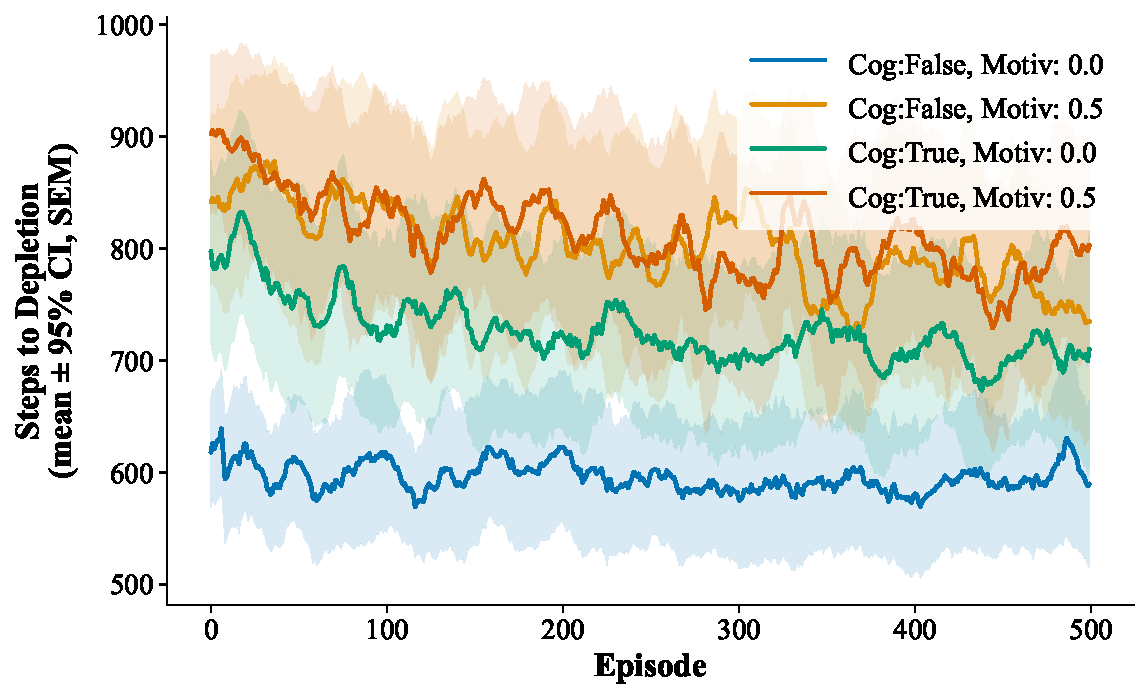
\includegraphics[width=0.8\textwidth]{figures/results/matrix_steps_trajectory}
  \caption{Episode length as a function of empathic properties across episodes. \textit{Cog}: ability to perceive others' emotions; \textit{Motiv}: empathic motivation.}
  \label{fig:matrix_steps_traj}
\end{figure}

\begin{figure}[H]
  \centering
  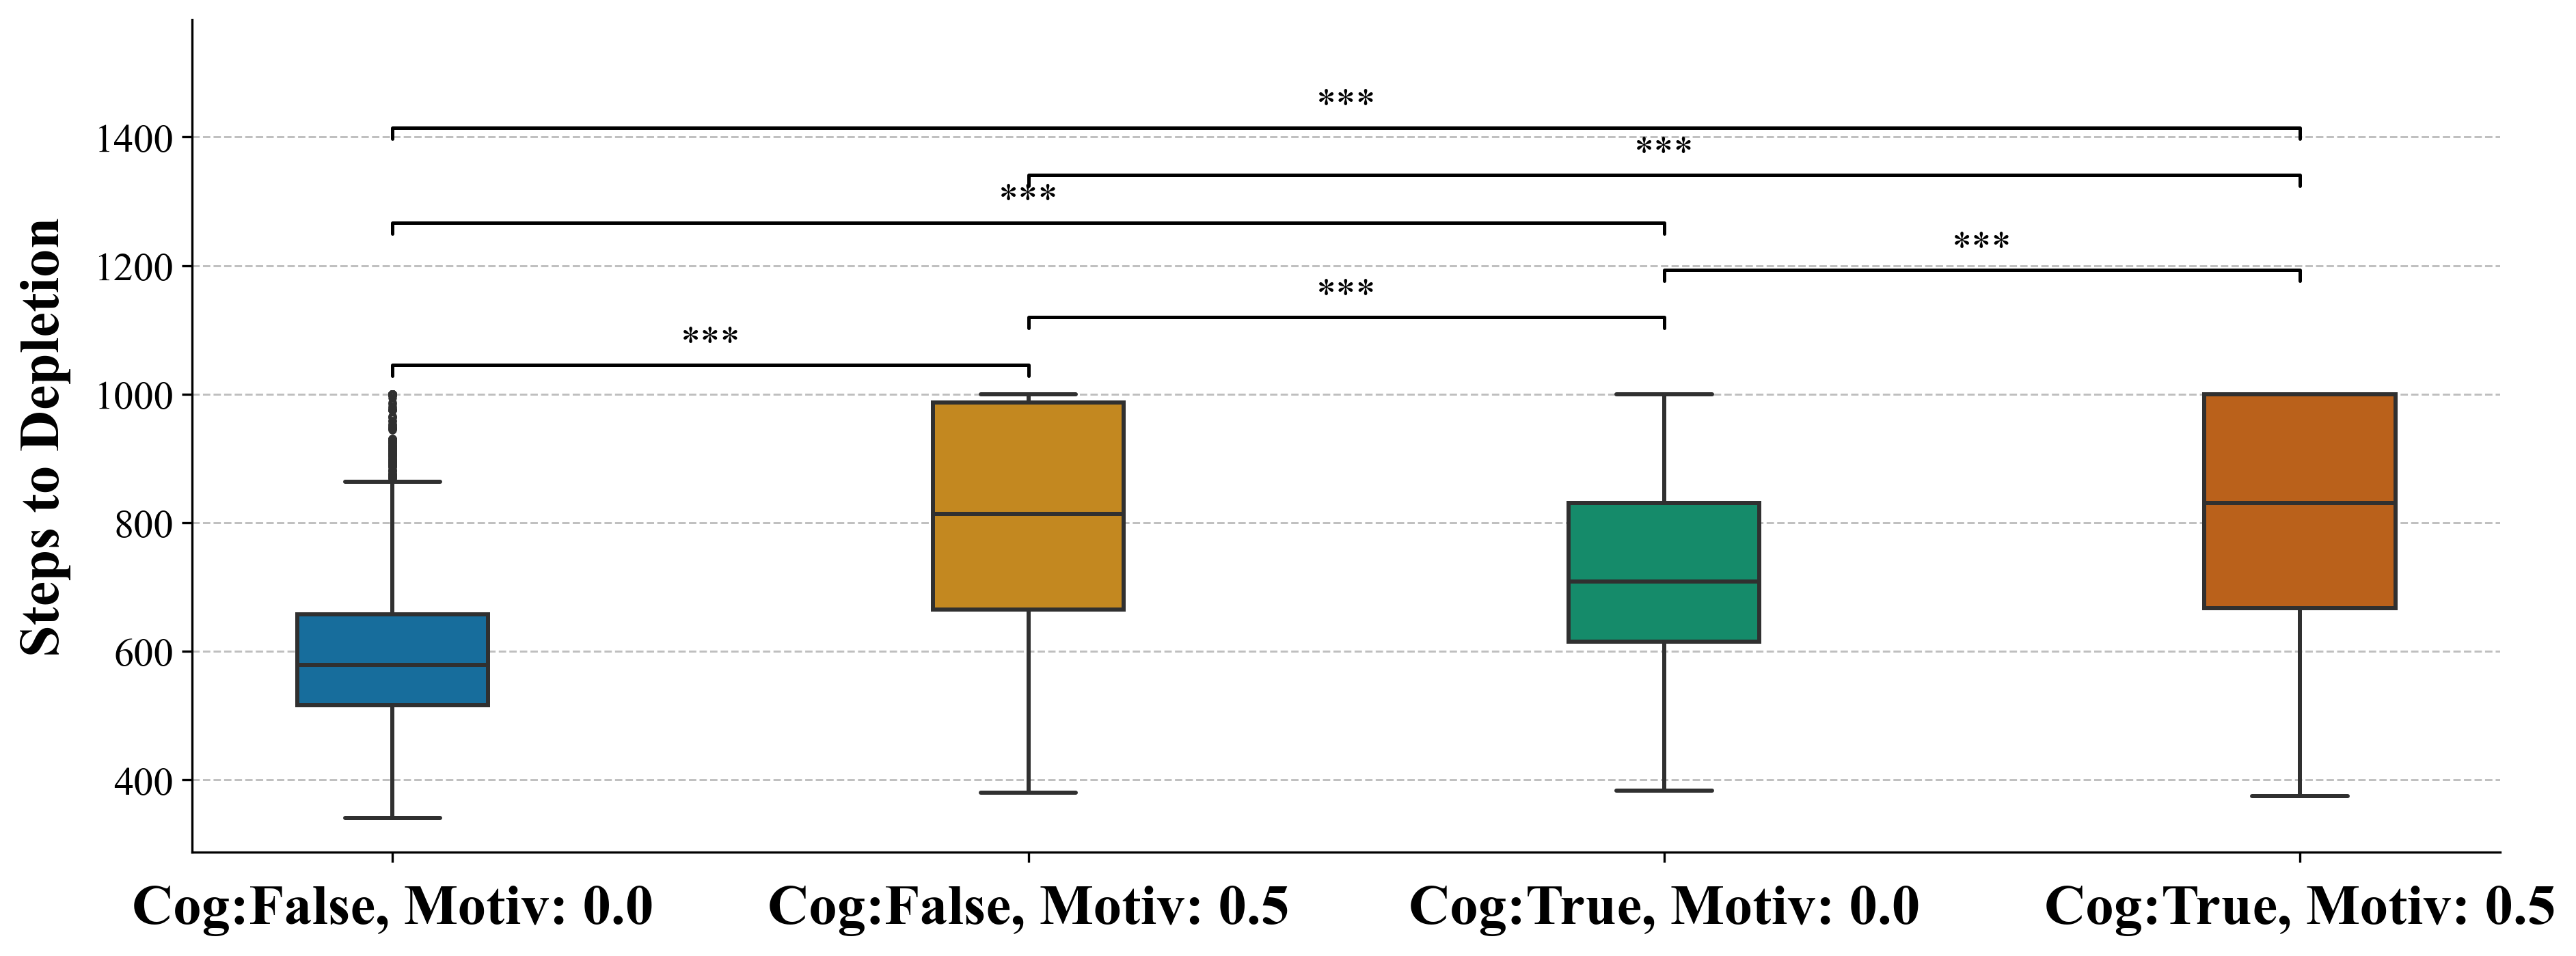
\includegraphics[width=\textwidth]{figures/results/full star matrix depletion.png}
  \caption{Episode length as a function of empathic properties, aggregated across episodes.}
  \label{fig:matrix_steps_box}
\end{figure}

A two-way ANOVA on episode length revealed significant main effects of emotion-perception ability ($F(1, 12) = 81.67$, $p < .001$, $\eta_p^2 = .87$) and empathic motivation ($F(1, 12) = 329.72$, $p < .001$, $\eta_p^2 = .96$). Specifically, simulations in which agents were able to perceive others' emotions showed greater sustainability than agents without this ability, and higher levels of empathic motivation were associated with longer episode durations. In addition, the interaction between the two factors was significant ($F(1, 12) = 57.69$, $p < .001$, $\eta_p^2 = .83$), following a sub-additive pattern: the benefit of each component was smaller when the other was already present, consistent with a ceiling effect on sustainability.

\subsubsection{Gini Coefficient.}
Figure~\ref{fig:matrix_gini_traj} shows the evolution of the Gini coefficient across episodes, and Fig.~\ref{fig:matrix_gini_box} presents the aggregated distributions.

\begin{figure}[H]
  \centering
  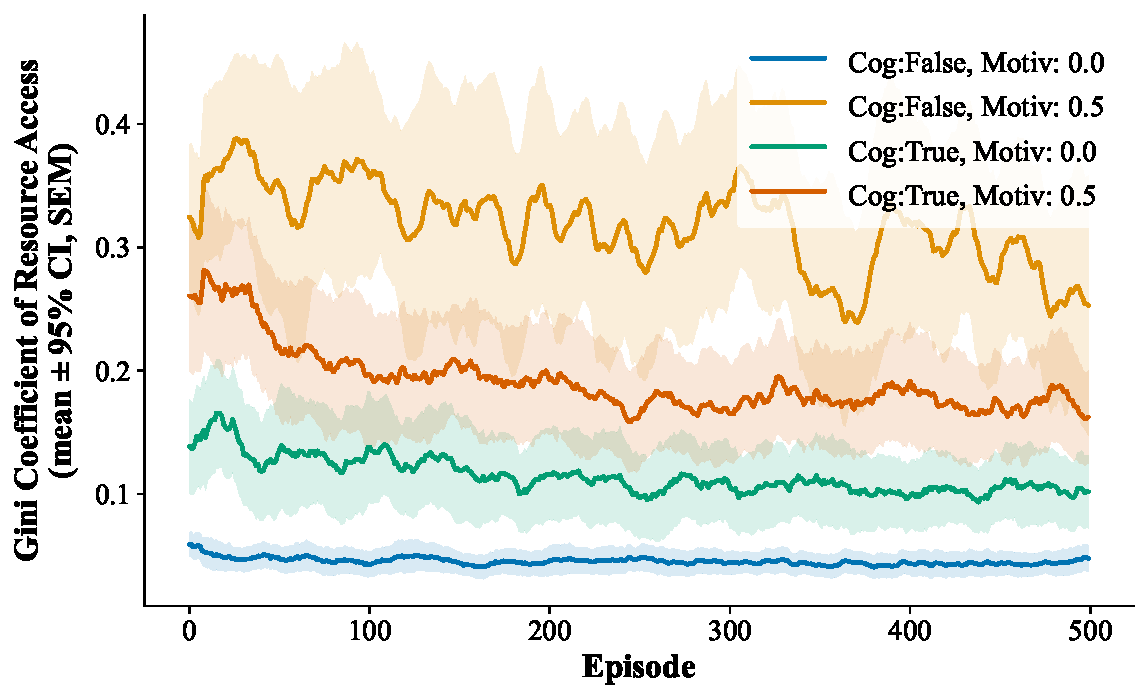
\includegraphics[width=0.8\textwidth]{figures/results/matrix_gini_trajectory.pdf}
  \caption{Fairness (Gini coefficient of resource access) as a function of empathic properties across episodes.}
  \label{fig:matrix_gini_traj}
\end{figure}

\begin{figure}[H]
  \centering
  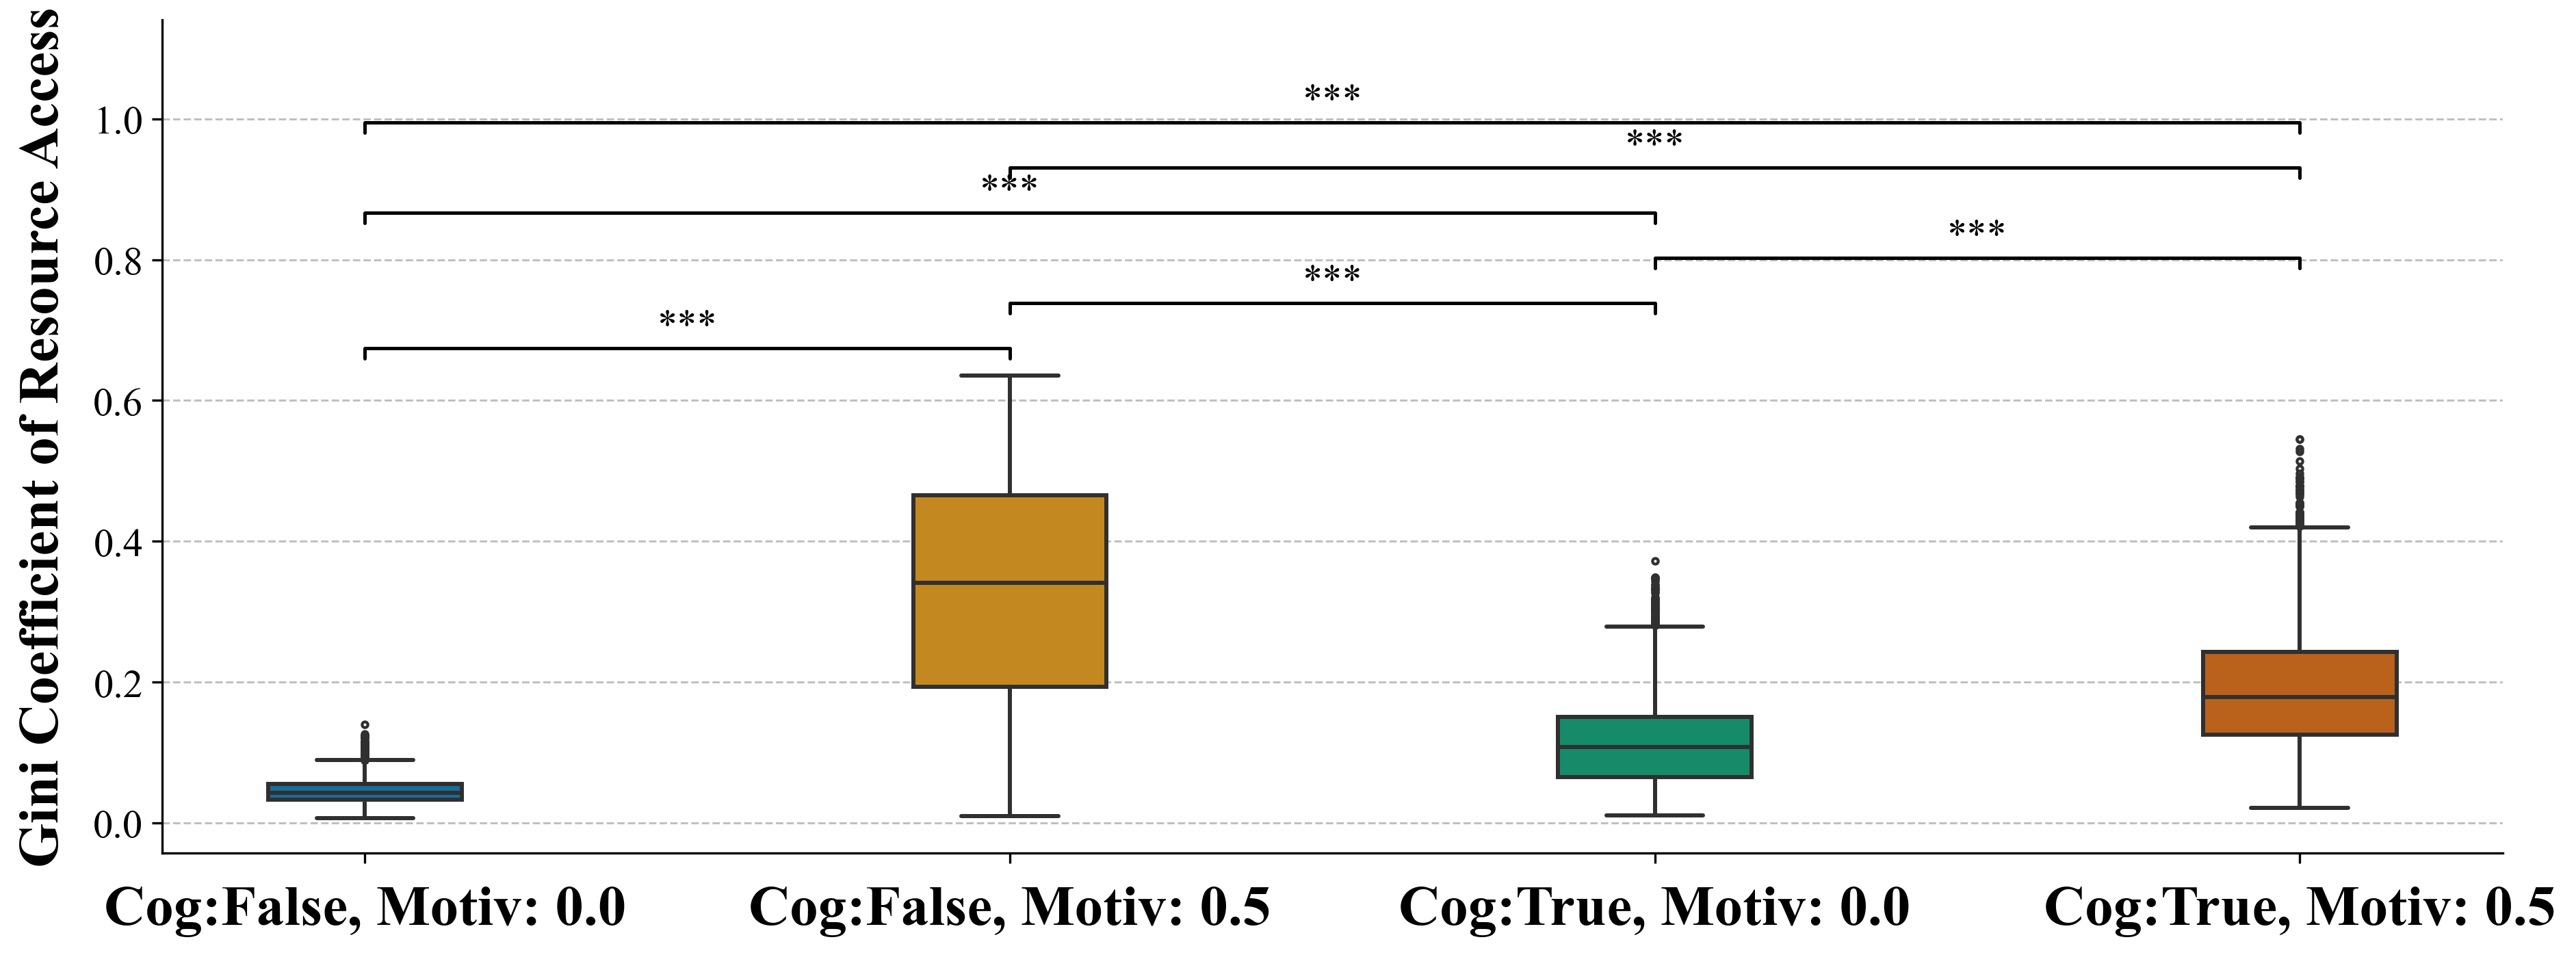
\includegraphics[width=\textwidth]{figures/results/full star matrix gini.png}
  \caption{Fairness (Gini coefficient of resource access) as a function of empathic properties, aggregated across episodes.}
  \label{fig:matrix_gini_box}
\end{figure}

A two-way ANOVA on the Gini coefficient revealed significant main effects of emotion-perception ability ($F(1, 12) = 12.13$, $p = .005$, $\eta_p^2 = .50$) and empathic motivation ($F(1, 12) = 458.68$, $p < .001$, $\eta_p^2 = .97$), qualified by a significant interaction between the two factors ($F(1, 12) = 145.64$, $p < .001$, $\eta_p^2 = .92$). Higher levels of empathic motivation were associated with higher Gini coefficients, whereas the effect of emotion perception depended on the motivational component: perceiving others' emotions increased inequality among non-empathic agents but substantially attenuated the inequality associated with motivational empathy.

\subsection{Study 2: More Altruistic Motivation, Less Depletion}

\subsubsection{Episode Length.}
Figure~\ref{fig:alpha_steps_traj} shows the evolution of episode length across episodes for varying degrees of altruism, and Fig.~\ref{fig:alpha_steps_box} presents the aggregated distributions.

\begin{figure}[H]
  \centering
  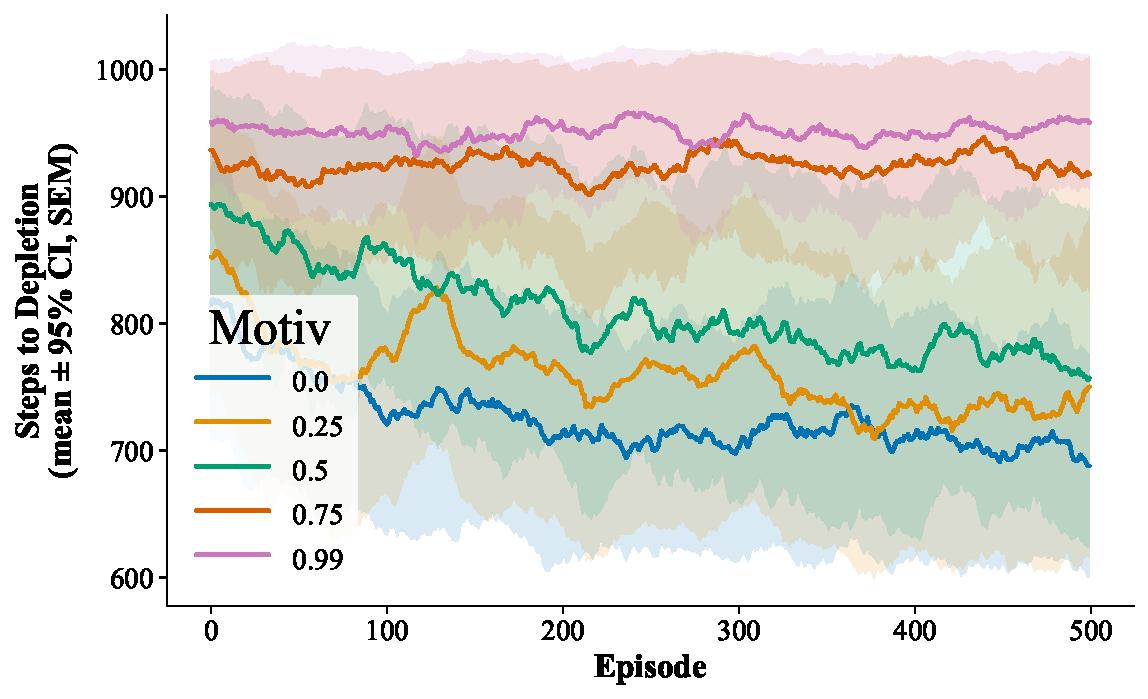
\includegraphics[width=0.8\textwidth]{figures/results/alpha_steps_trajectory}
  \caption{Episode length as a function of the degree of altruism ($\alpha_e$) across episodes.}
  \label{fig:alpha_steps_traj}
\end{figure}

\begin{figure}[H]
  \centering
  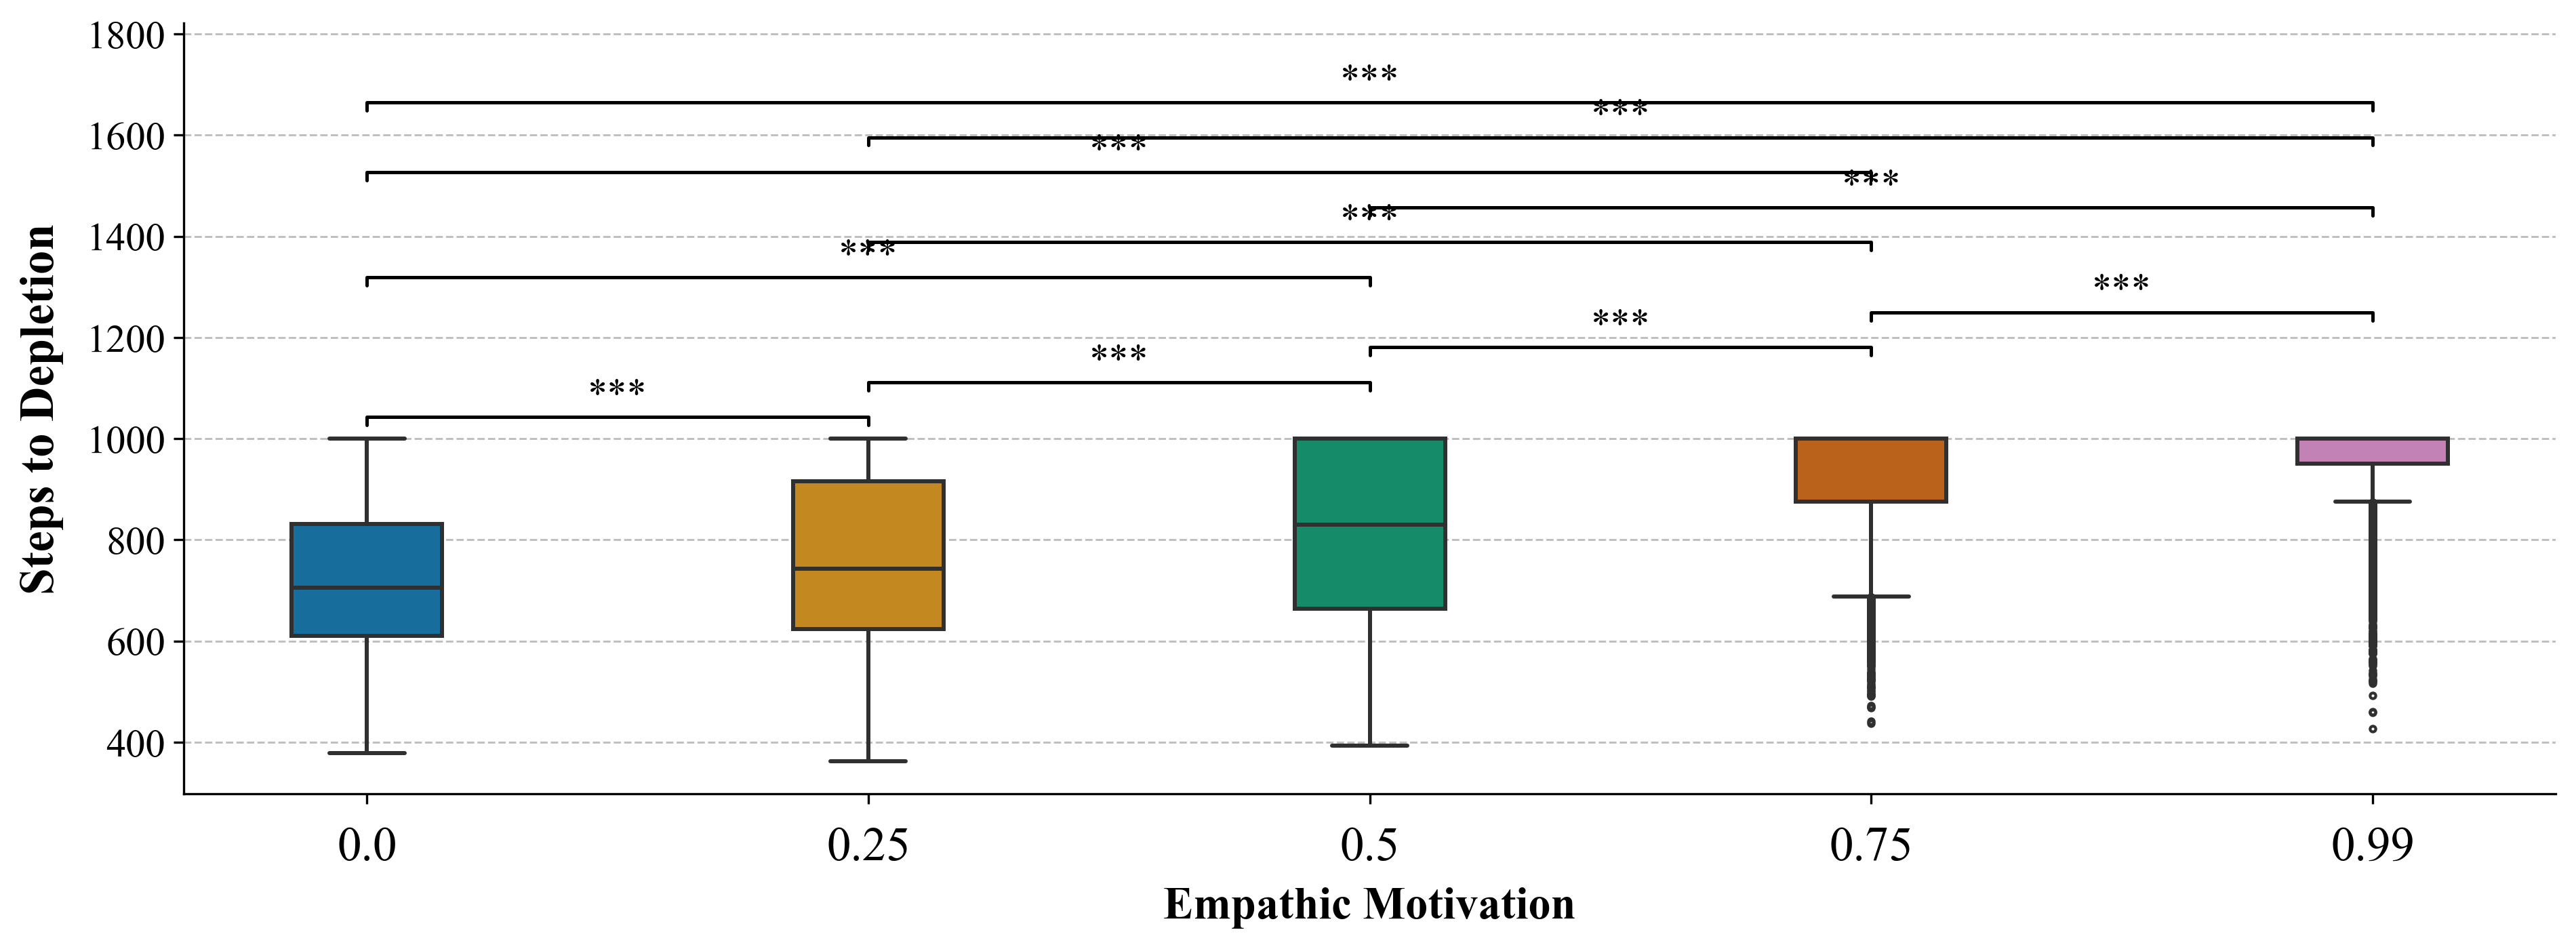
\includegraphics[width=\textwidth]{figures/results/full star alpha depletion.png}
  \caption{Episode length as a function of the degree of altruism ($\alpha_e$), aggregated across episodes.}
  \label{fig:alpha_steps_box}
\end{figure}

A positive Spearman correlation was found between the number of steps before depletion and the empathic motivation parameter ($r_s(18) = .92$, $p < .001$), indicating that simulations with agents that have higher levels of altruistic motivation were associated with longer-lasting episodes before depletion occurred.

\subsubsection{Gini Coefficient.}
Figure~\ref{fig:alpha_gini_traj} shows the evolution of the Gini coefficient across episodes, and Fig.~\ref{fig:alpha_gini_box} presents the aggregated distributions.

\begin{figure}[H]
  \centering
  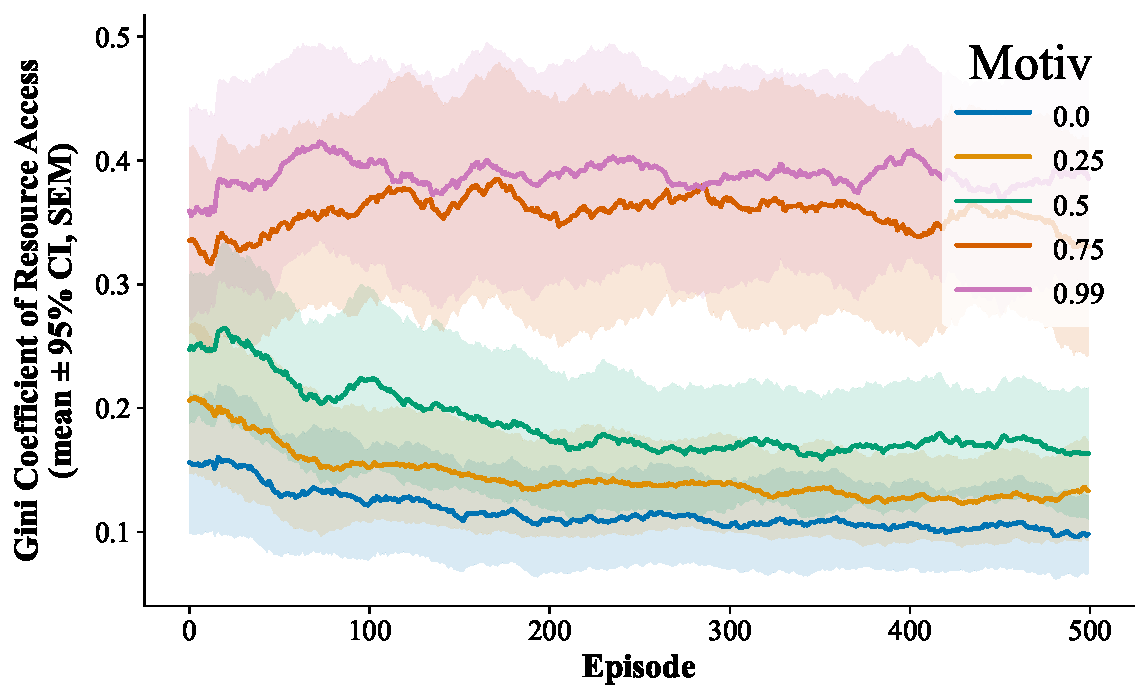
\includegraphics[width=0.8\textwidth]{figures/results/alpha_gini_trajectory}
  \caption{Fairness (Gini coefficient of resource access) as a function of the degree of altruism ($\alpha_e$) across episodes.}
  \label{fig:alpha_gini_traj}
\end{figure}

\begin{figure}[H]
  \centering
  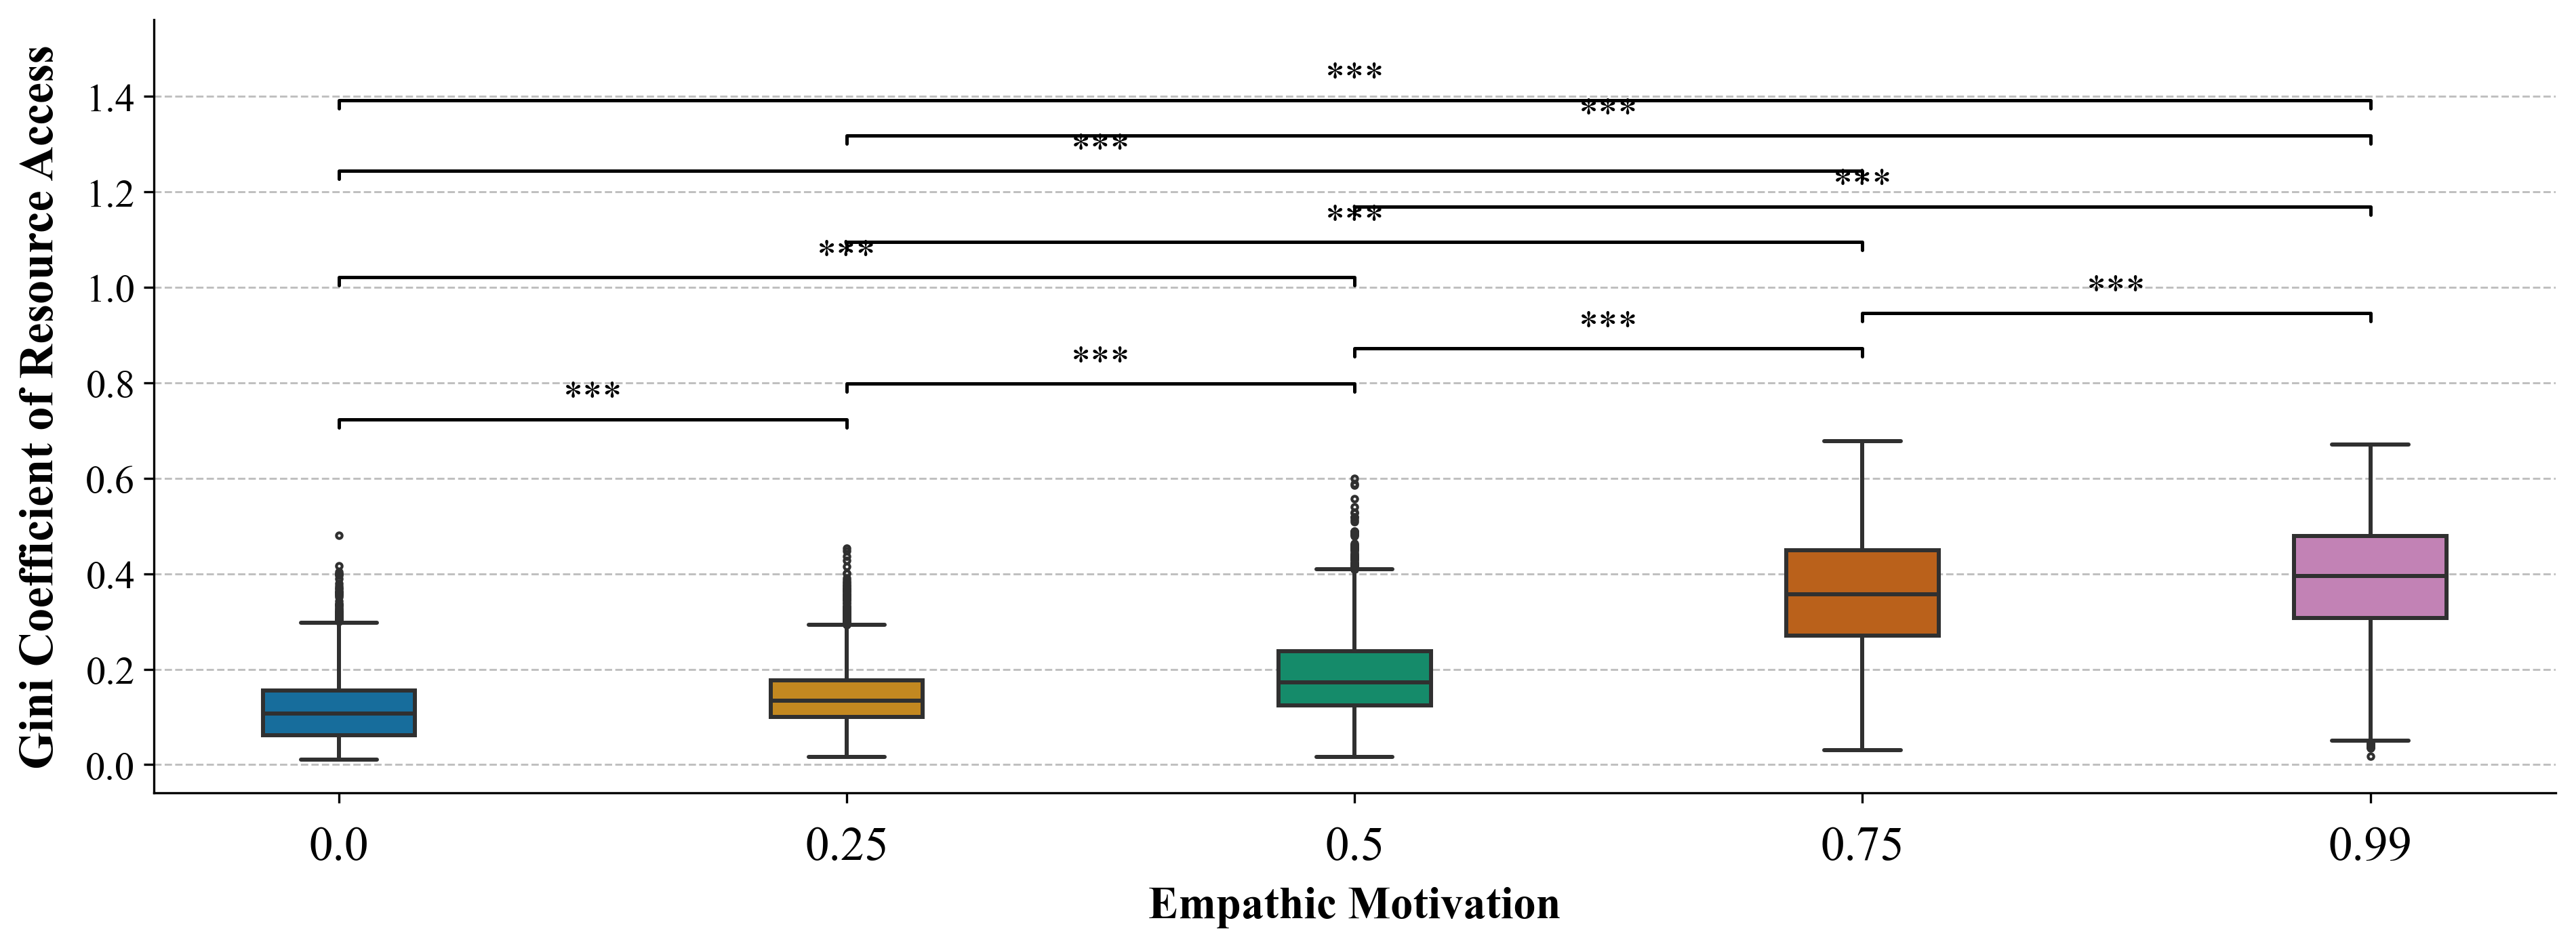
\includegraphics[width=\textwidth]{figures/results/full star alpha Gini.png}
  \caption{Fairness (Gini coefficient of resource access) as a function of the degree of altruism ($\alpha_e$), aggregated across episodes.}
  \label{fig:alpha_gini_box}
\end{figure}

A positive Spearman correlation was found between the Gini coefficient and the empathic motivation parameter ($r_s(18) = .96$, $p < .001$), indicating that simulations with agents that have higher levels of altruistic motivation were associated with less equitable resource distribution.


\newpage
\section{Discussion}
\subsection{Interpretation of results}

Using multi-agent reinforcement learning simulations to investigate the role of two empathy components---cognitive and motivational---in promoting pro-environmental behaviors, we hypothesized that the sustainability of the system dynamics, measured by episode length, would be enhanced by both components of empathy. Furthermore, along with Du et al. \cite{du_2024}, we expected fairness (equality in resource acquisition) to be favored by empathy.

\subsubsection{Empathy and Sustainability}
In line with (TH1), Study 1 revealed significant main effects of the presence of both cognitive and motivational empathy on episode length, as well as a significant, sub-additive interaction between the two components. Motivational empathy emerged as the primary driver of sustainability: simulations in which agents received an empathic reward were associated with substantially longer episodes before depletion, regardless of access to affective signals. The small magnitude of the difference between the Blind/Empathic and Full Empathy conditions suggests that motivational empathy alone may be sufficient to sustain the resource at a comparable level, and that cognitive access to others' emotional states only marginally amplifies this effect under simple binary action selection. Additionally, in line with (TH3), Study 2 confirmed this dose-response relationship, with a strong positive correlation between the degree of altruistic motivation and resource sustainability.

These results are consistent with the hypothesis of empathy-altruism \cite{batson1997perspective,Batson01041991,batson2022empathy}, which proposes that empathic concern, an emotional response oriented to other people that is congruent with the perceived welfare of another, is the primary driver of prosocial behavior. As a process, empathic concern is triggered by two conditions: a belief that another is in need, and an intrinsic valuation of that other's welfare. Once elicited, it generates a motivational state in which egoistic and altruistic motivations interact through a hedonic calculus, ultimately shaping action selection. Our framework directly instantiates this process: the valence signal broadcast by each agent is congruent with its consumption satisfaction, and the empathic reward received by peers is a direct function of this signal. When others signal distress (negative valence), agents with a nonzero empathic reward coefficient are penalized for consuming, functionally replicating the trigger of empathic concern. The empathic weight itself models the hedonic/utility calculus at the heart of the hypothesis, interpolating between purely egoistic (altruistic weight $\alpha_e = 0$) and predominantly altruistic ($\alpha_e \rightarrow 1$) motivational states.

This operationalization also maps onto the distinction between reactive empathy and perspective-taking. Reactive empathy, feeling for another by experiencing an emotion of congruent valence \cite{batson1997perspective}, is captured by the motivational component: agents experience a reward signal of the same valence as their peers' affective states, increasing their empathic concern. Perspective-taking, by contrast, improves the adjustment to a more complex state space. In our framework, access to others' affective signals (cognitive empathy condition) provides agents with the perceptual input needed for such estimation. This may explain why the interaction between cognitive and motivational empathy on sustainability is sub-additive: perspective-taking refines the expression of altruistic motivation but is not itself a source of that motivation. Together, this aligns with dual-interest theory \cite{lynneTheoreticalFoundationEmpathy2016} and cognitive-affective-motivational conceptualizations of empathy \cite{decetyNeuralPathwaysDevelopment2015,dewaalMammalianEmpathyBehavioural2017}. That said, depletion remained nearly systematic across all conditions, suggesting that empathy as operationalized here delays but does not prevent the Tragedy of the Commons. This points to the need for complementary mechanisms, such as internal representations of resource state or institutional constraints, to achieve genuine sustainability \cite{ostromGeneralFrameworkAnalyzing2009,vanlangeHowWeCan2008}.

\subsubsection{Empathy and Fairness}
Contrary to (TH2), both cognitive and motivational empathy were associated with higher Gini coefficients, indicating greater inequality in resource distribution. Study 2 further confirmed this pattern, with an opposite result to (TH4) with altruistic motivation strongly and positively correlated with inequality.

At first glance, this contradicts the empathy-altruism hypothesis, which would predict that other-regarding motivation promotes equitable as well as sustainable outcomes. However, the hypothesis specifies that empathic concern targets welfare, not equality \cite{Batson01041991}. The discrete set of emotions constituting empathic concern is oriented toward the perceived need of another, not toward distributive justice between all others. In a shared resource environment, an agent experiencing empathic concern may consistently restrain its own consumption to benefit peers, but this self-restraint does not compel equal distribution across all agents. Rather, as agents follow heterogeneous learning trajectories under identical algorithms, differential consumption rates can emerge, producing objective inequality as an unintended byproduct of other-regarding motivation.

The reward structure reinforces this dynamic. Agents who consume less still achieve comparable aggregate rewards because the social component of the reward compensates for reduced personal gain. This reduces sensitivity to self-disadvantageous inequity: since perceived aggregate utility remains stable regardless of consumption asymmetries, there is less pressure to equalize access \cite{heInfluenceEmpathicConcern2022}. Empathic concern may thus decouple sustainability from fairness.

The significant interaction observed in Study 1 offers a partial qualification: the inequality associated with motivational empathy was attenuated when agents could perceive others' affective states. Within the empathy-altruism framework, this is interpretable through the role of perspective-taking: access to others' valence signals improves the accuracy of need estimation \cite{batson1997perspective}, allowing agents to direct their care more precisely and reducing the polarization of consumption patterns. Without affective signals, reactive empathy remains diffuse and undirected; with them, agents can modulate restraint in response to specific others' perceived states, producing a more needs-responsive and comparatively less unequal distribution \cite{moreno-casasEthicsCareTragedy2021}.

These results raise broader theoretical questions: to what extent can empathy offset personal disadvantage? Are self-interest and social rewards integrated into a unified utility signal or processed as separate domains? And how would these dynamics change if the resource were essential for survival, altering the valence and intensity of the empathic concern elicited? Developing precise computational models with categorical distinctions between empathy, normative influence, and instrumental reasoning remains essential to advance our understanding of pro-environmental behavior.


\subsection{Limitations and future work}
\subsubsection{Limitations}
Simulation parameters were selected through brute-force exploration, following an approach inspired by Perolat et al.\ (2017) \cite{perolatMultiagentReinforcementLearning2017}. The simulations were carried out under conditions where a sufficient number of agents was known to reliably produce resource depletion, allowing the observation of emergent behaviors under scarcity.

Several features of the current design limit direct transferability to human behavior. First, the affective signaling mechanism relies on a linear mapping from consumption rate to valence, which may not capture the nonlinear dynamics of human emotional experience. Alternative mappings,  such as sigmoid transformations or bio-inspired computational models of emotion \cite{gannouniAdaptiveEmotionDetection2020,joffilyEmotionalValenceFreeenergy2013},  could yield richer affective signals and increase the plausibility of our framework as a model of human empathic processing. Second, agents in the current simulations discount future rewards at a rate of $\gamma = 0.99$, meaning they weigh near-future outcomes nearly as heavily as immediate ones. This contrasts with human temporal discounting, where future rewards are systematically devalued, an effect that intensifies under uncertainty \cite{storyDiscountingFutureReward2024}. Testing lower discount factors would improve ecological validity by assessing whether the sustainability benefits of empathy hold under more human-like temporal preferences. Third, research suggests that empathic valuation and behavioral investment in others' needs decay over time \cite{colemanIntertemporalEmpathyDecline2024}, a dynamic not currently captured in our framework. Fourth, even resource consumption in real-world contexts is rarely binary; human decisions involve graded, context-sensitive trade-offs that a two-action model cannot fully represent.

\subsubsection{Future Directions}
Beyond addressing these limitations, several extensions are planned. Moving to a 2D spatial environment would allow the study of proximity-based empathic dynamics and more realistic foraging behaviors. Exploring alternative reward functions, including non-linear formulations and need-sensitive consumption penalties, would allow a more fine-grained test of the conditions under which empathy promotes both sustainability and fairness. Finally, fitting these simulations to data from analogous human behavioral tasks could provide parameter estimates with greater empirical grounding, bridging the gap between computational modeling and psychological theory.
While this work provides insights into the role of empathy in pro-environmental behaviors, it is not sufficient. The transferability of our findings to human and other contexts is limited.

\subsection{Conclusion}
This study presents a novel multi-agent reinforcement learning framework for investigating the computational role of empathy in common-pool resource dilemmas. By operationalizing empathy through affective signaling observation (cognitive component) and reward shaping (motivational component), we observed that both components contribute independently and interactively to resource sustainability. Motivational empathy emerged as the primary driver of reduced overconsumption, while cognitive empathy modulated the fairness of resource distribution. Contrary to our initial hypotheses, higher empathic motivation was associated with greater inequality, an effect partially mitigated by access to peers' affective states.

These findings provide initial computational grounding for empathy-based theories of pro-environmental behavior and confirm that empathy can be a relevant mechanism for cooperative resource management beyond purely institutional or normative approaches. Future work should extend this framework to richer environments, including 2D spatial settings, continuous action spaces, and resources with regenerative dynamics, and to explore how these simulated results can be connected to human behavioral data through model fitting.


\begin{credits}
\subsubsection{\ackname} This work was supported by the European Commission's CAVAA Project (EIC 101071178) and by a French government grant managed by the Agence Nationale de la Recherche as part of the France 2030 program, reference ANR-24-EXEN-0001 (PEPR eNSEMBLE / COMCOMBBr). The authors would like to warmly thank Arnaud Blanchard, Nicolas Bredèche, Laura Cohen, Maël Crépey and Clément Moulin-Frier for useful discussions.

\subsubsection{\discintname} The authors have no competing interests to declare that are relevant to the content of this article.
\end{credits}

\newpage
\appendix

\section{Common Simulation Parameters}
\label{app:simparams}

\begin{table}[h]
\centering
\begin{tabular}{lll}
\hline
\textbf{Parameter} & \textbf{Symbol} & \textbf{Value} \\
\hline
Number of agents      & $N$     & $6$    \\
Initial resource      & $R_0$   & $500$  \\
Episodes per run      & ---     & $500$  \\
Max steps per episode & ---     & $1000$ \\
Replications per condition & --- & $4$  \\
\hline
\end{tabular}
\caption{Common simulation parameters shared across all conditions and studies.}
\label{tab:simparams}
\end{table}

\section{DQN Hyperparameters}
\label{app:hyperparams}

\begin{table}[h]
\centering
\begin{tabular}{lll}
\hline
\textbf{Parameter} & \textbf{Symbol} & \textbf{Value} \\
\hline
Learning rate         & $\alpha$         & $0.001$ \\
Discount factor       & $\gamma$         & $0.99$  \\
Initial exploration   & $\varepsilon_0$  & $1.0$   \\
Minimum exploration   & $\varepsilon_{\min}$ & $0.01$ \\
Exploration decay     & $\varepsilon_{\text{decay}}$ & $0.995$ \\
Replay batch size     & ---              & $16$    \\
Target update freq.   & ---              & $5$ steps \\
Hidden layer size     & ---              & $64$ ($\times 2$) \\
\hline
\end{tabular}
\caption{DQN hyperparameters shared across all agents.}
\label{tab:hyperparams}
\end{table}

Agents follow an $\varepsilon$-greedy policy:
\begin{equation}
    a_i^t =
    \begin{cases}
        \text{random action} & \text{with prob. } \varepsilon_t, \\
        \arg\max_{a} Q(s_t, a;\, \theta) & \text{with prob. } 1 - \varepsilon_t,
    \end{cases}
\end{equation}
with $\varepsilon_t$ decayed as
$\varepsilon_{t+1} = \max(\varepsilon_{\min},\, \varepsilon_t \cdot \varepsilon_{\text{decay}})$.

The Q-network is updated by minimising the mean squared Bellman error over
sampled experience batches, using target values:
\begin{equation}
    y_t = r_t + \gamma \cdot \max_{a'} Q(s_{t+1}, a';\, \theta^{-})
\end{equation}
where $\theta^{-}$ denotes the parameters of the periodically-frozen target network.

\newpage

%
% ---- Bibliography ----
%
% BibTeX users should specify bibliography style 'splncs04'.
% References will then be sorted and formatted in the correct style.
%

\begin{thebibliography}{99}

\bibitem{hardinTragedyCommonsPopulation1968}
Hardin, G.: The tragedy of the commons. \textit{Science} \textbf{162}(3859), 1243--1248 (1968)

\bibitem{patelModellingCooperationCompetition2021}
Patel, A., Williams, H., Ramaswamy, N.: Modelling cooperation and competition using multi-agent reinforcement learning. \textit{Journal of Artificial Intelligence Research} \textbf{70}, 321--355 (2021)

\bibitem{ostromRevisitingCommonsLocal1999}
Ostrom, E.: Revisiting the commons: local lessons, global challenges. \textit{Science} \textbf{284}(5412), 278--282 (1999)

\bibitem{perolatMultiagentReinforcementLearning2017}
Perolat, J., Leibo, J.Z., Zambaldi, V., Kramár, J., Sunehag, P., Legg, S.: A multi-agent reinforcement learning method for impression. In: Proceedings of the 34th International Conference on Machine Learning, vol. 70, pp. 2749--2757 (2017)

\bibitem{nashEquilibriumPointsPerson1950}
Nash, J.F.: Equilibrium points in n-person games. \textit{Proceedings of the National Academy of Sciences} \textbf{36}(1), 48--49 (1950)

\bibitem{vanlangeHowWeCan2008}
Van Lange, P.A.M., Joireman, J., Parks, C.D., Van Dijk, E.: The psychology of social dilemmas: A review. \textit{Organizational Behavior and Human Decision Performance} \textbf{120}(2), 125--141 (2008)

\bibitem{gronauerMultiagentDeepReinforcement2022}
Grönauer, B., Klaus, R.: Multi-agent deep reinforcement learning: a survey. \textit{Artificial Intelligence Review} \textbf{55}(2), 895--943 (2022)

\bibitem{wangEvolvingIntrinsicMotivations2018}
Wang, J.X., Hughes, E., Fernando, C., Czarnecki, J.M., Duvenaud, D., Leibo, J.Z.: Evolving intrinsic motivations for altruistic behavior. In: Proceedings of the 17th International Conference on Autonomous Agents and Multiagent Systems, pp. 683--692 (2018)

\bibitem{zhuDeepMultiagentReinforcement2019}
Zhu, Q., Tembine, H., Bas, T.: Distributed game play in multi-population multi-agent reinforcement learning. \textit{IEEE Transactions on Games} \textbf{11}(2), 174--185 (2019)

\bibitem{kosterModelfreeConventionsMultiagent2020}
Köster, R., Hadfield-Menell, D., Everett, R., Sunehag, P., Leibo, J.Z.: Spurious reciprocity in machine learning. \textit{Advances in Neural Information Processing Systems} \textbf{33}, 17102--17114 (2020)

\bibitem{massiModelbasedModelfreeReplay2022}
Massi, B., Szita, I., Ernst, D.: Model-based versus model-free reinforcement learning. \textit{Annual Review of Biomedical Data Science} \textbf{5}, 29--51 (2022)

\bibitem{rosemanEmotionalBehaviorsEmotivational2011}
Roseman, I.J.: Emotional behaviors, emotivational goals, emotion strategies: Multiple levels of organization integrate variable inputs and activate coordinated outputs. \textit{Emotion Review} \textbf{3}(4), 434--443 (2011)

\bibitem{russellCoreAffectPsychological2003}
Russell, J.A.: Core affect and the psychological construction of emotion. \textit{Psychological Review} \textbf{110}(1), 145--172 (2003)

\bibitem{broschCommentAppraisingBrain2013}
Brosch, T., Pourtois, G., Sander, D.: From appraisal to saliency: The Amplification of individual differences in emotional reactivity. \textit{Frontiers in Psychology} \textbf{4}, 357 (2013)

\bibitem{moorsPowerGoalDirectedProcesses2017}
Moors, A., Ellsworth, P.C., Scherer, K.R., Frijda, N.H.: Appraisal theories of emotion: State of the art and future development. \textit{Emotion Review} \textbf{9}(4), 319--324 (2017)

\bibitem{lynneTheoreticalFoundationEmpathy2016}
Lynne, G.D.: Toward a theoretical foundation for socio-egoistic value theory and stated preference methods. \textit{Journal of Environmental Economics and Management} \textbf{78}, 4--19 (2016)

\bibitem{cuffEmpathyReviewConcept2016}
Cuff, B.M., Brown, S.J., Taylor, L., Howat, D.J.: Empathy: A review of the concept. \textit{Emotion Review} \textbf{8}(2), 144--153 (2016)

\bibitem{bosnjakovicEmpathyConceptsTheories2018}
Bosnakovic, E., Rueckert, L., Theis, F.J.: Neural mechanisms of empathy in schizophrenia. \textit{Neuroscience} \textbf{375}, 100--118 (2018)

\bibitem{dewaalMammalianEmpathyBehavioural2017}
de Waal, F.B.: Mammalian empathy. \textit{Nature} \textbf{534}(7607), 455--456 (2017)

\bibitem{bekkaliPutativeMirrorNeuron2021}
Bekkali, S., Mazzocco, K., Aucouturier, J.L., Bufalari, I., Friston, K., Daunizeau, J.: Neural correlates of theory of mind in an immersive virtual reality social interaction. \textit{Scientific Reports} \textbf{11}(1), 17906 (2021)

\bibitem{boniniMirrorNeurons302022}
Bonini, L., Maranesi, M., Livi, A., Fogassi, L., Rozzi, S.: Space encoding in two hierarchically organized sensorimotor areas. \textit{Nature Reviews Neuroscience} \textbf{23}(1), 5--20 (2022)

\bibitem{bernhardtNeuralBasisEmpathy2012}
Bernhardt, B.C., Singer, T.: The neural basis of empathy. \textit{Annual Review of Neuroscience} \textbf{35}, 1--23 (2012)

\bibitem{dvashTheoryMindEmpathy2014}
Dvash, J., Gilam, G., Zagoory-Sharon, O., Talmon, R., Hendler, T.: Neuroscientific evidence for ritualistic behavior in autism. \textit{Current Biology} \textbf{20}(8), 738--739 (2014)

\bibitem{decetyEmergenceEmpathyDevelopmental2021}
Decety, J., Fotopoulou, A.: Social neuroscience of empathy. \textit{Current Opinion in Psychology} \textbf{37}, 87--92 (2021)

\bibitem{decetyNeuralPathwaysDevelopment2015}
Decety, J., Michalska, K.J.: Neurodevelopmental changes in the circuits underlying empathy and sympathy from childhood to adulthood. \textit{Developmental Science} \textbf{13}(6), 886--899 (2015)

\bibitem{Batson01041991}
Batson, C.D., Ahmad, N., Tsang, J.A.: Empathic joy and the empathy-altruism hypothesis. \textit{Journal of Personality and Social Psychology} \textbf{61}(3), 413--426 (1991)

\bibitem{batson2022empathy}
Batson, C.D.: Empathy and altruism. In: The Oxford Handbook of Social Neuroscience, pp. 263--272 (2022)

\bibitem{ostromGeneralFrameworkAnalyzing2009}
Ostrom, E.: A general framework for analyzing sustainability of social-ecological systems. \textit{Science} \textbf{325}(5939), 419--422 (2009)

\bibitem{rabinovichProtectingCommonsPredictors2020}
Rabinowitz, D., Tory, S.P., Rouhani, S., Sagi, D.: Protecting the commons: Predictors of group-beneficial resource management. \textit{Proceedings of the National Academy of Sciences} \textbf{117}(37), 22872--22877 (2020)

\bibitem{cuadradoRoleProsocialnessTrust2017}
Cuadrado, J.R., Brañas-Garza, P., Rodriguez-Lara, I.: Social preferences and cooperation in multiplayer dilemmas. \textit{Applied Economics} \textbf{49}(52), 5360--5372 (2017)

\bibitem{decaroSynergisticEffectsVoting2015}
De Caro, O., Sap, E., Scuotto, V.: Synergistic effects of voting rules and communication on cooperation. \textit{Journal of Economic Behavior \& Organization} \textbf{113}, 88--104 (2015)

\bibitem{decaroMotivationalFoundationsCommunication2021}
De Caro, O., Carboni, O., D'Adda, G.: Motivational foundations of communication. \textit{Games} \textbf{12}(1), 17 (2021)

\bibitem{fornaraExtendedValueBeliefNormTheory2020}
Fornara, F., Pattitoni, P., Mura, M., Strazzera, E.: Predicting intention to donate money for climate change mitigation: Value, beliefs, and attitudes. \textit{Journal of Environmental Psychology} \textbf{69}, 101433 (2020)

\bibitem{guoResidentialElectricityConsumption2018}
Guo, J., Ruan, S., Li, S., Zhu, H.: Residential electricity consumption behavior: Evidence from China. \textit{Renewable and Sustainable Energy Reviews} \textbf{81}, 2670--2677 (2018)

\bibitem{liWhatInfluencesIndividuals2019}
Li, X., Wang, Y., Ge, J.: What influences individuals' intentions to purchase green vehicles? An integrated analysis of the influencing factors. \textit{Transportation Research Part D: Transport and Environment} \textbf{68}, 214--229 (2019)

\bibitem{sussmanProEnvironmentalValuesMatter2016}
Sussman, R., Gifford, R.: Causation beliefs, environmental concern, and activism. \textit{Environment and Behavior} \textbf{48}(2), 259--282 (2016)

\bibitem{sternValuebeliefnormTheorySupport1999}
Stern, P.C., Dietz, T., Guagnano, G.A.: A brief inventory of values. \textit{Educational and Psychological Measurement} \textbf{53}(3), 667--674 (1999)

\bibitem{ajzenTheoryPlannedBehavior1991}
Ajzen, I.: The theory of planned behavior. \textit{Organizational Behavior and Human Decision Performance} \textbf{50}(2), 179--211 (1991)

\bibitem{moreno-casasEthicsCareTragedy2021}
Moreno-Casas, P., Vázquez-Campos, J., Francés-Gómez, P.: Ethics of care and tragedy of the commons. \textit{Environmental Ethics} \textbf{43}(1), 77--92 (2021)

\bibitem{tomaselloTwoKeySteps2012}
Tomasello, M., Carpenter, M.: Two key steps in the evolution of human cooperation. \textit{Current Anthropology} \textbf{53}(6), 673--692 (2012)

\bibitem{tomaselloOriginsHumanCooperation2013}
Tomasello, M., Melis, A.P., Tomasello, M.: The evolution of cooperation. \textit{Philosophical Transactions of the Royal Society B: Biological Sciences} \textbf{364}(1518), 665--666 (2013)

\bibitem{yuEmotionalMultiagentReinforcement2015}
Yu, C., Zhang, M., Ren, F.: Emotional multi-agent reinforcement learning in strategy games. \textit{Neurocomputing} \textbf{170}, 73--83 (2015)

\bibitem{thiermannMotivatingIndividualsSocial2020}
Thiermann, F.B., Sheate, W.R.: Motivating individuals for pro-environmental behaviour through a dual-interest model. \textit{Sustainability} \textbf{12}(20), 8576 (2020)

\bibitem{mnih2015}
Mnih, V., Kavukcuoglu, K., Silver, D., et al.: Human-level control through deep reinforcement learning. \textit{Nature} \textbf{529}(7587), 529--533 (2015)

\bibitem{du_2024}
Du, Y., Meyn, S., Basar, T.: Learning to cooperate in complex networked multiagent systems. \textit{IEEE Transactions on Automatic Control} \textbf{69}(4), 2345--2360 (2024)

\bibitem{heInfluenceEmpathicConcern2022}
He, Z., Zhang, H., Gao, X., Li, Y.: The influence of empathic concern on fairness in social dilemmas. \textit{Frontiers in Psychology} \textbf{13}, 823456 (2022)

\bibitem{batson1997perspective}
Batson, C.D., Ahmad, N., Powell, A.A.: Empathy and altruism. \textit{International Handbook of Multigenerational Legacies of Trauma}, 263--272 (1997)

\bibitem{gannouniAdaptiveEmotionDetection2020}
Gannouni, S., Abed, A.B.: Adaptive emotion detection and recognition from facial expressions. \textit{Multimedia Tools and Applications} \textbf{79}(17), 11877--11894 (2020)

\bibitem{joffilyEmotionalValenceFreeenergy2013}
Joffily, M., Coricelli, G.: The behavioral and neuroscientific impact of count and continuity on emotional experience. \textit{Social Cognitive and Affective Neuroscience} \textbf{8}(4), 395--404 (2013)

\bibitem{storyDiscountingFutureReward2024}
Story, G.W., Vlaev, I., Seymour, B., et al.: Does temporal discounting predict prosocial behavior? \textit{Proceedings of the Royal Society B: Biological Sciences} \textbf{281}(1778), 20231622 (2024)

\bibitem{colemanIntertemporalEmpathyDecline2024}
Coleman, S., Mitchell, D., Jackson, J.: Intertemporal empathy decline and long-term prosocial commitments. \textit{Journal of Behavioral Decision Making} \textbf{37}(1), e2847 (2024)

\end{thebibliography}

\end{document}
